% Name: Braiding and its inverse
% Description: The braiding of two wires, its inverse, and the equation that says they cancel.
% Tags: braiding, inverse, braided category

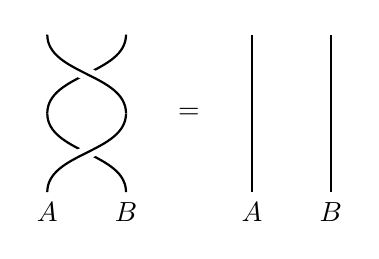
\begin{tikzpicture}[thick, baseline=(current bounding box.center)]
  % c_{A,B} followed by its inverse
  \draw (1,0) .. controls (1,0.5) and (0,0.5) .. (0,1);
  \draw[white, line width=5pt] (0,0) .. controls (0,0.5) and (1,0.5) .. (1,1);
  \draw (0,0) .. controls (0,0.5) and (1,0.5) .. (1,1);
  \draw (0,1) .. controls (0,1.5) and (1,1.5) .. (1,2);
  \draw[white, line width=5pt] (1,1) .. controls (1,1.5) and (0,1.5) .. (0,2);
  \draw (1,1) .. controls (1,1.5) and (0,1.5) .. (0,2);
  \node[below] at (0,0) {$A$};
  \node[below] at (1,0) {$B$};
  \node at (1.8,1) {$=$};
  \draw (2.6,0) node[below] {$A$} -- (2.6,2);
  \draw (3.6,0) node[below] {$B$} -- (3.6,2);
\end{tikzpicture}
